\subsection{Completed historical pilot and paired operating-value results}
\label{sec:copper-completed-results}
The ten-date pilot admits 7 dates and 6 chronological pairs, with 480 common model forecasts and 375 observations on persistence support. Its gaps are the actual gaps between admitted dates, not assumed daily steps. The remaining 21 gold reference dates were not acquired in this pilot; their absence from this experiment does not establish unavailable history. The table records the quality exclusions rather than manufacturing a balanced panel.

\begin{table}[H]
\centering
\small
\caption{Actual copper pilot coverage; dates below 64 eligible quotes or three expiries are excluded.}
\label{tab:copper-temporal-coverage}
\begin{tabularx}{\textwidth}{@{}Xrrrr@{}}
\toprule
Date & Retrieved & Eligible & Expiries & Admitted \\
\midrule
2026-07-09 & 100 & 75 & 5 & Yes \\
2026-07-10 & 104 & 53 & 5 & No \\
2026-07-20 & 79 & 74 & 5 & Yes \\
2026-07-31 & 75 & 18 & 2 & No \\
2026-08-03 & 73 & 41 & 5 & No \\
2026-08-12 & 88 & 82 & 6 & Yes \\
2026-08-21 & 100 & 86 & 6 & Yes \\
2026-08-31 & 97 & 87 & 6 & Yes \\
2026-09-01 & 97 & 65 & 6 & Yes \\
2026-09-02 & 99 & 86 & 6 & Yes \\
\bottomrule
\end{tabularx}
\end{table}

Admitted origin--target pairs (calendar-day gaps): 2026-07-09 to 2026-07-20 (11); 2026-07-20 to 2026-08-12 (23); 2026-08-12 to 2026-08-21 (9); 2026-08-21 to 2026-08-31 (10); 2026-08-31 to 2026-09-01 (1); 2026-09-01 to 2026-09-02 (1).
The reported RMSE is the equal-weight mean of target-date RMSEs. The $R^2$ instead compares sums of target-date MSEs on each declared support. Root-mean MSE and observation-weighted pooled scores are retained separately in the reproducibility outputs.
\begin{table}[H]
\centering
\small
\caption{Copper conditional temporal IV tests: date-equal aggregation. The persistence comparison uses its inside-hull support; fixed-origin robustness freezes the first admitted fit.}
\label{tab:copper-temporal-models}
\begin{tabularx}{\textwidth}{@{}Xrrr@{}}
\toprule
Model & Rolling RMSE (bp) & $R^2_{mean}$ & $R^2_{persist}$ \\
\midrule
Black--76 & 106.48 & 0.002 & -1.294 \\
Heston & 71.46 & 0.458 & -0.422 \\
Bates--Poisson & 70.49 & 0.465 & -0.389 \\
Bates--Hawkes & 67.65 & 0.518 & -0.208 \\
\bottomrule
\end{tabularx}
\end{table}

\begin{table}[H]
\centering
\small
\caption{Fixed-first-origin robustness on the same 480 model forecasts; persistence support contains 333 observations. Structural parameters remain frozen at 2026-07-09.}
\label{tab:copper-fixed-origin}
\begin{tabularx}{\textwidth}{@{}Xrrr@{}}
\toprule
Model & Fixed RMSE (bp) & $R^2_{mean}$ & $R^2_{persist}$ \\
\midrule
Black--76 & 115.38 & 0.001 & -0.345 \\
Heston & 111.94 & -0.050 & -0.282 \\
Bates--Poisson & 90.94 & 0.337 & 0.193 \\
Bates--Hawkes & 92.56 & 0.334 & 0.182 \\
\bottomrule
\end{tabularx}
\end{table}

In the rolling test, no model improves on observed-surface persistence on its common support. The fixed-origin check gives positive persistence-relative point estimates for Bates--Poisson (0.193), Bates--Hawkes (0.182); its different origin gaps and support do not establish stable superiority. Reserved-strike interpolation results remain a separate experiment. Fixed-origin targets overlap the rolling sample and do not constitute independent replication. With only 6 forecast pairs, these estimates support a preliminary diagnostic, not a stable economic model ranking or a claim of statistical superiority.

\begin{table}[H]
\centering
\small
\caption{Paired five-year operating-value proxies, USD billion, no terminal value, independent gold/copper scenarios and 8,192 common paths. Monte Carlo SE concerns only the mean increment.}
\label{tab:copper-paired-value}
\begin{tabularx}{\textwidth}{@{}Xrrrr@{}}
\toprule
Model & Gold only & Gold + copper & Increment & MC SE \\
\midrule
Black--76 & 14.857 & 17.484 & 2.627 & 0.023 \\
Heston & 14.847 & 17.465 & 2.618 & 0.039 \\
Bates--Poisson & 14.746 & 17.409 & 2.663 & 0.040 \\
Bates--Hawkes & 14.776 & 17.417 & 2.641 & 0.037 \\
\bottomrule
\end{tabularx}
\end{table}

The valuation uses a full eligible 2 September copper fit with that date's Treasury curve. Its parameters are used only in the final scenario, not retroactively in historical origins. The gold baseline remains frozen, including its company-actual/eight-mine-forecast scope break. Parameter uncertainty, operating-plan uncertainty and the unreconciled corporate cash-flow bridge are outside the Monte Carlo SE. A temporal IV test does not validate those missing economic quantities.

\begin{figure}[H]
\centering
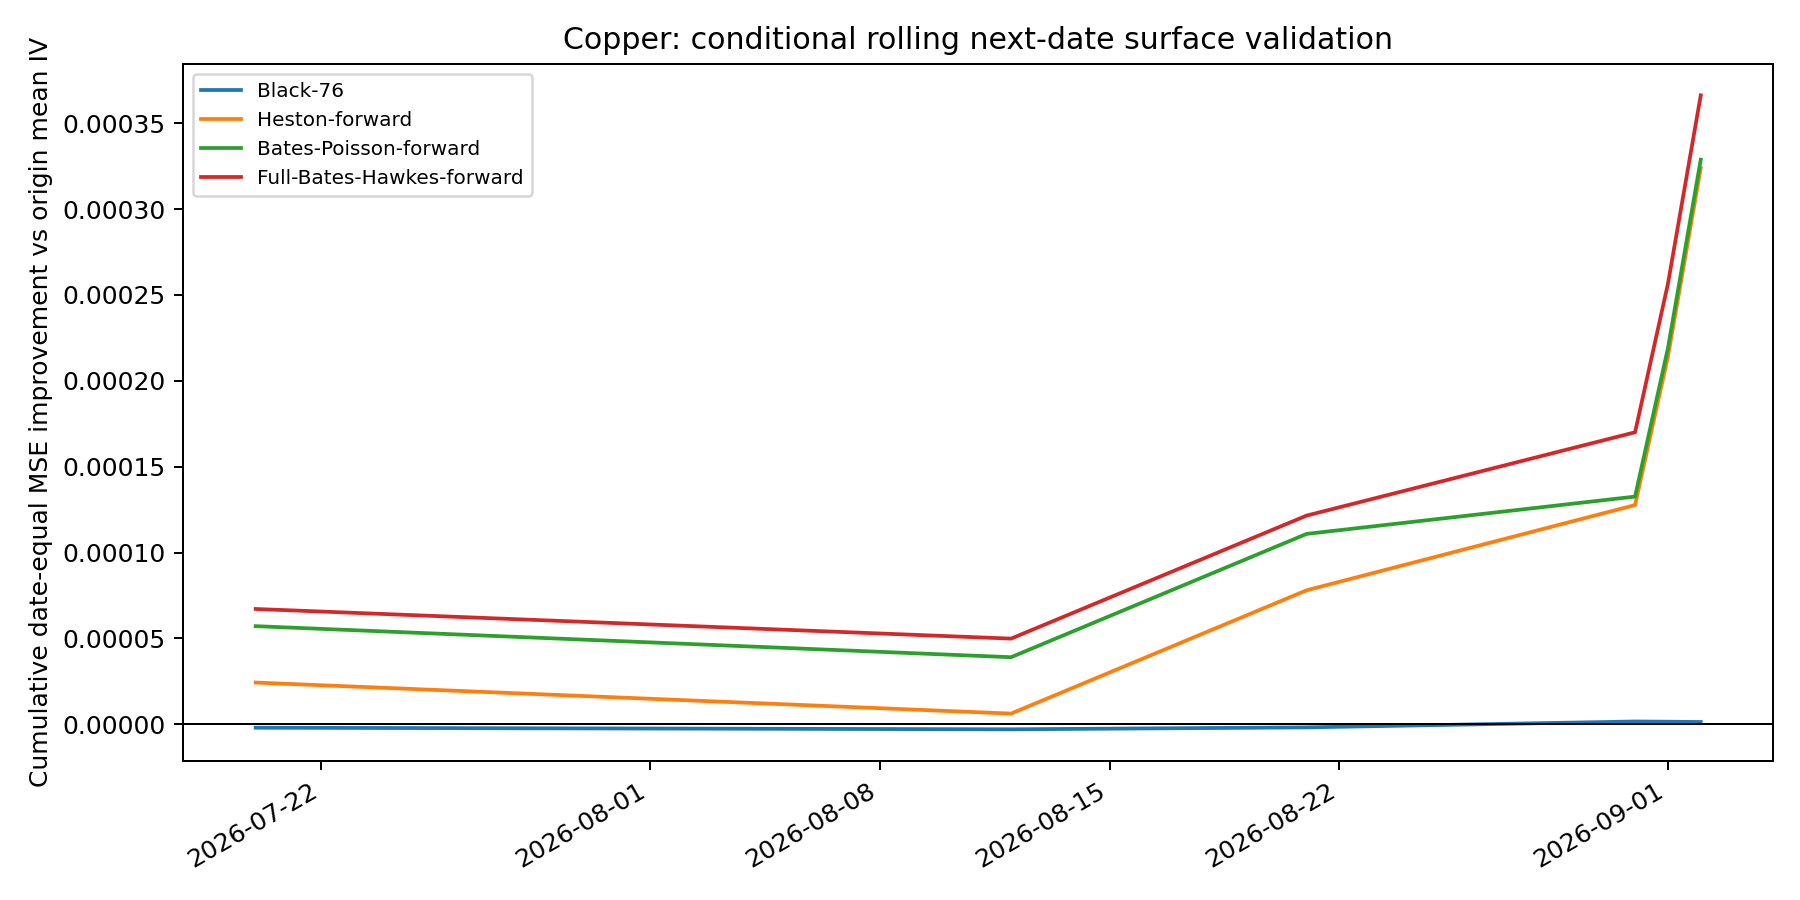
\includegraphics[width=.96\textwidth]{img/copper/copper_temporal_oos.png}
\caption{Cumulative date-equal MSE improvement against origin-mean IV. Only actual admitted targets enter; elapsed gaps are preserved. Positive improvement against this benchmark need not imply improvement against surface persistence.}
\label{fig:copper-temporal-oos}
\end{figure}
